\documentclass[11pt]{report}

\usepackage[utf8]{inputenc}
\usepackage[T1]{fontenc}
\usepackage[french]{babel}
\usepackage{graphicx}
\usepackage{float}
\usepackage{amsmath}
\usepackage{caption}
\usepackage[a4paper, margin=2.5cm]{geometry}

\title{A Cross-Sectional Study of a One-Day Intraday Reversal Strategy}
\author{Valentin Lourme}
\date{\today}

\begin{document}

\maketitle
\tableofcontents

\chapter{Introduction}

L'objectif de cette étude est d'analyser les mouvements économiques réels des actifs. Les prix ajustés sont donc utilisés afin d'éliminer les ruptures artificielles provoquées par les splits et les dividendes, qui ne correspondent pas à des mouvements de marché.

\chapter{Construction de la stratégie One-Day Intraday Reversal}

\section{Explications de la stratégie One-Day Intraday Reversal}

La stratégie proposée dans cette étude repose sur l'hypothèse que les mouvements intrajournaliers exceptionnellement importants ont tendance à être suivis, lors de la séance suivante, par un mouvement de correction. L'objectif est ainsi d'identifier les journées présentant un déplacement anormal du prix puis d'exploiter un éventuel phénomène de \textit{mean reversion}.

Pour chaque actif, on dispose quotidiennement du prix d'ouverture $O_t$, du plus haut $H_t$, du plus bas $L_t$ ainsi que du prix de clôture $C_t$. Le mouvement intrajournalier absolu est défini par

$$
M_t=
\left|
\frac{C_t}{O_t}-1
\right|,
$$

qui mesure l'amplitude du déplacement réalisé entre l'ouverture et la clôture de la séance.

Afin de tenir compte des effets calendaires, la volatilité attendue est estimée séparément pour chaque jour de la semaine. Ainsi, la volatilité attendue d'un lundi est calculée uniquement à partir des quatorze lundis précédents. Cette construction permet d'éviter de comparer directement des journées présentant naturellement des comportements différents.

La volatilité attendue est alors estimée par

$$
\frac{1}{14}
\sum_{i=1}^{14}
M_{t_i},
$$

où les observations $t_i$ correspondent aux quatorze dernières séances appartenant au même jour de la semaine que la date (t).

À partir de cette estimation, deux bornes dynamiques sont construites autour du prix d'ouverture :

$$
O_t
\left(
1+\widehat{M}_t
\right),
$$

$$
O_t
\left(
1-\widehat{M}_t
\right),
$$

où $UB_t$ et $LB_t$ désignent respectivement la borne supérieure et la borne inférieure attendues pour la séance.

Un signal de trading est ensuite généré selon la règle suivante :

$$
S_t=
\begin{cases}
-1, & \text{si } H_t > O_t\left(1+\widehat{M}_t\right)
      \text{ et }
      L_t \geq O_t\left(1-\widehat{M}_t\right), \\[0.35cm]
+1, & \text{si } L_t < O_t\left(1-\widehat{M}_t\right)
      \text{ et }
      H_t \leq O_t\left(1+\widehat{M}_t\right), \\[0.35cm]
0, & \text{sinon.}
\end{cases}
$$

Autrement dit, un signal vendeur est généré lorsqu'une hausse intrajournalière dépasse le mouvement statistiquement attendu, tandis qu'un signal acheteur est produit lorsqu'une baisse anormalement importante est observée. Les journées durant lesquelles les deux bornes sont franchies simultanément sont volontairement exclues, celles-ci correspondant généralement à des épisodes de volatilité exceptionnelle pour lesquels le sens du mouvement devient ambigu.

Le signal détecté au cours de la séance (t-1) est exécuté à l'ouverture de la séance (t). Cette hypothèse garantit que toutes les informations utilisées pour générer le signal sont effectivement disponibles avant l'ouverture de la position.

Le rendement intrajournalier de la séance est défini par

$$
\frac{C_t}{O_t}-1,
$$

et le rendement quotidien de la stratégie est donné par


$$
S_{t-1}\times R_t.
$$

Ainsi, un signal vendeur $S_{t-1}=-1$ correspond à une vente à l'ouverture suivie d'un rachat à la clôture de la séance, tandis qu'un signal acheteur $S_{t-1}=1$ correspond à une position longue ouverte à l'ouverture puis liquidée à la clôture.

Cette construction conduit à une stratégie entièrement systématique, ne reposant sur aucun ajustement ex post ni sur aucune optimisation spécifique à un actif. Le seul paramètre utilisé est une estimation historique de la volatilité intrajournalière récente. Les chapitres suivants chercheront à déterminer dans quelles conditions cette hypothèse de retournement intrajournalier est effectivement vérifiée, quels actifs présentent une sensibilité particulière à ce signal et quelles conditions de marché favorisent son efficacité.

\newpage

\section{comparaison de l'application de ODIR sur differents actifs}

Cette première partie vise à évaluer la performance globale de la stratégie de \textit{One-Day Intraday Reversal} sur l'ensemble de l'univers d'investissement étudié. Avant de chercher à comprendre pourquoi certains actifs réagissent plus favorablement que d'autres au signal de retournement, il est nécessaire de vérifier que la stratégie présente un comportement statistiquement intéressant à l'échelle de l'univers complet.

L'analyse débute par l'étude de la distribution des ratios de Sharpe annualisés obtenus sur chacun des actifs. Cette représentation permet d'apprécier simultanément la performance moyenne de la stratégie, la dispersion des résultats ainsi que l'existence éventuelle d'une hétérogénéité entre les actifs.

\begin{figure}[H]
\centering
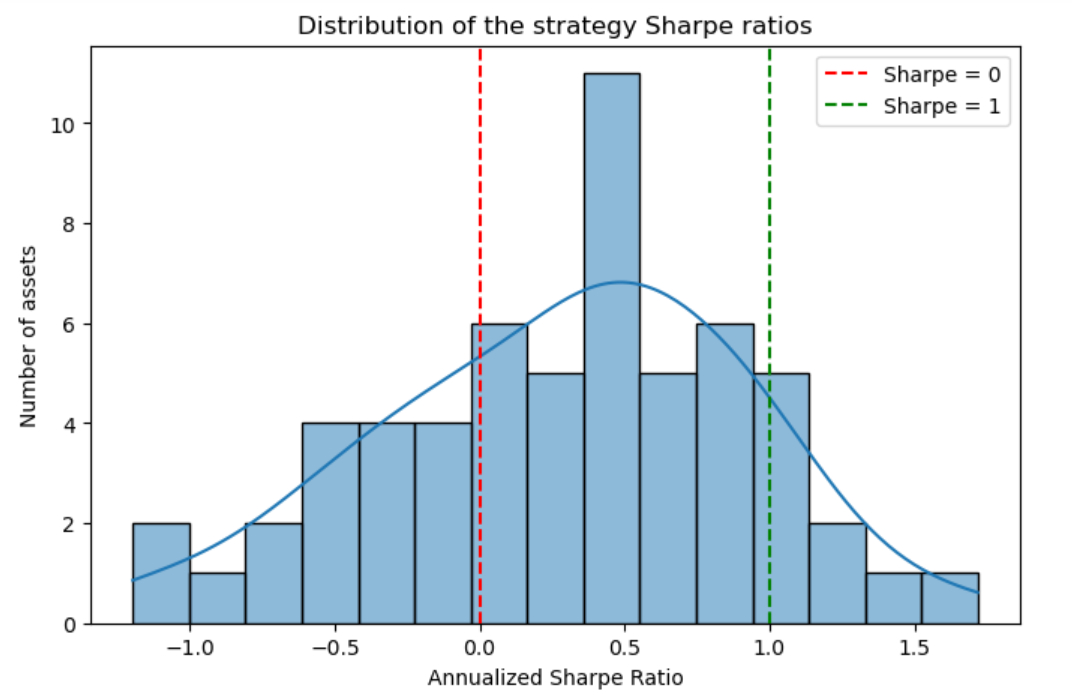
\includegraphics[width=0.80\textwidth]{Illustrations/SharpeHistogram.png}
\caption{Distribution des ratios de Sharpe annualisés obtenus sur l'ensemble des actifs étudiés.}
\label{fig}
\end{figure}

Cette première analyse répond notamment aux questions suivantes :

\begin{enumerate}
\item La stratégie génère-t-elle un alpha positif en moyenne ?
\item Les performances sont-elles homogènes au sein de l'univers étudié ?
\item Quelle proportion des actifs présente un ratio de Sharpe économiquement significatif ?
\end{enumerate}

La Figure~\ref{fig} met en évidence la dispersion des performances entre les différents actifs. Afin d'identifier précisément les titres sur lesquels la stratégie est la plus efficace, les ratios de Sharpe sont ensuite classés par ordre décroissant.

\begin{figure}[H]
\centering
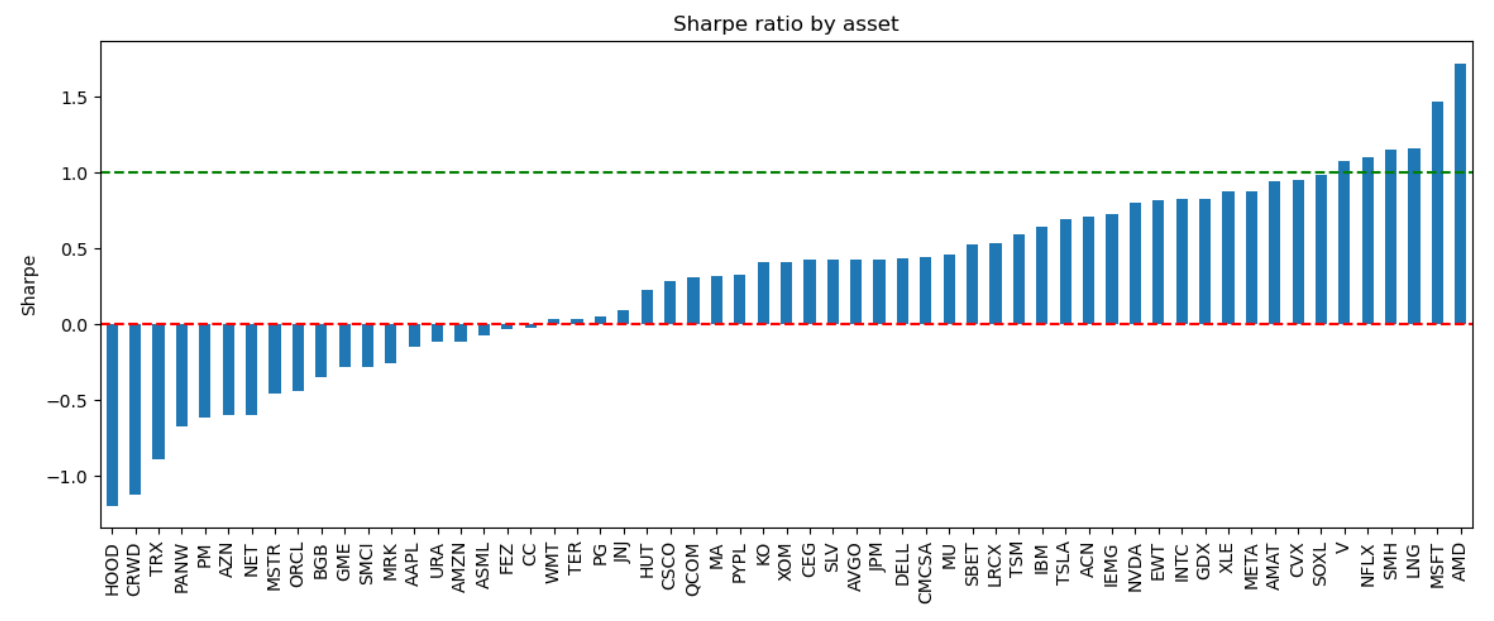
\includegraphics[width=\textwidth]{Illustrations/SharpeByAsset.png}
\caption{Classement des actifs selon leur ratio de Sharpe annualisé.}
\label{fig}
\end{figure}

Les résultats précédents mettent en évidence une forte hétérogénéité des performances obtenues par la stratégie. Alors que certains actifs, tels qu'AMD, MSFT ou LNG, affichent des ratios de Sharpe supérieurs à 1, voire supérieurs à 1.5, d'autres, comme HOOD, CRWD ou TRX, présentent des performances fortement négatives avec des ratios de Sharpe inférieurs à -1.

Cette dispersion montre que la stratégie de \textit{One-Day Intraday Reversal} ne constitue pas une stratégie universellement profitable. Son efficacité dépend manifestement de caractéristiques propres aux actifs sur lesquels elle est appliquée.

Une première hypothèse naturelle consiste à attribuer cette différence de comportement au secteur d'activité. Les résultats ne semblent toutefois pas confirmer cette intuition. Au sein d'un même secteur, des actifs peuvent présenter des comportements radicalement différents. Le secteur des semi-conducteurs en fournit une illustration : AMD et NVDA affichent des performances particulièrement élevées, tandis qu'ASML présente un ratio de Sharpe proche de zéro malgré une exposition au même environnement économique.

Cette observation suggère que la variable explicative recherchée ne relève probablement pas du secteur d'activité mais de propriétés statistiques intrinsèques aux actifs. Certaines séries de prix semblent naturellement plus réceptives à un signal de retournement intrajournalier que d'autres.

Cette constatation constitue le point de départ de la seconde partie de cette étude. L'objectif n'est plus uniquement d'évaluer la performance de la stratégie, mais d'identifier les caractéristiques quantitatives qui rendent un actif favorable à son application. Au-delà des propriétés propres aux actifs, cette analyse cherchera également à déterminer si certaines conditions de marché renforcent ou affaiblissent l'efficacité du signal de retournement.

\chapter{Identification des actifs et des conditions de marché favorables}


La seconde partie de ce travail cherchera ainsi à répondre à cette question en étudiant les propriétés statistiques susceptibles de prédire la sensibilité d'un actif à un signal de retournement intrajournalier.
\end{document}
